\clearpage
\section*{Appendix: Supplementary Outputs of the Same Python Run}

\begin{figure}[H]
\centering
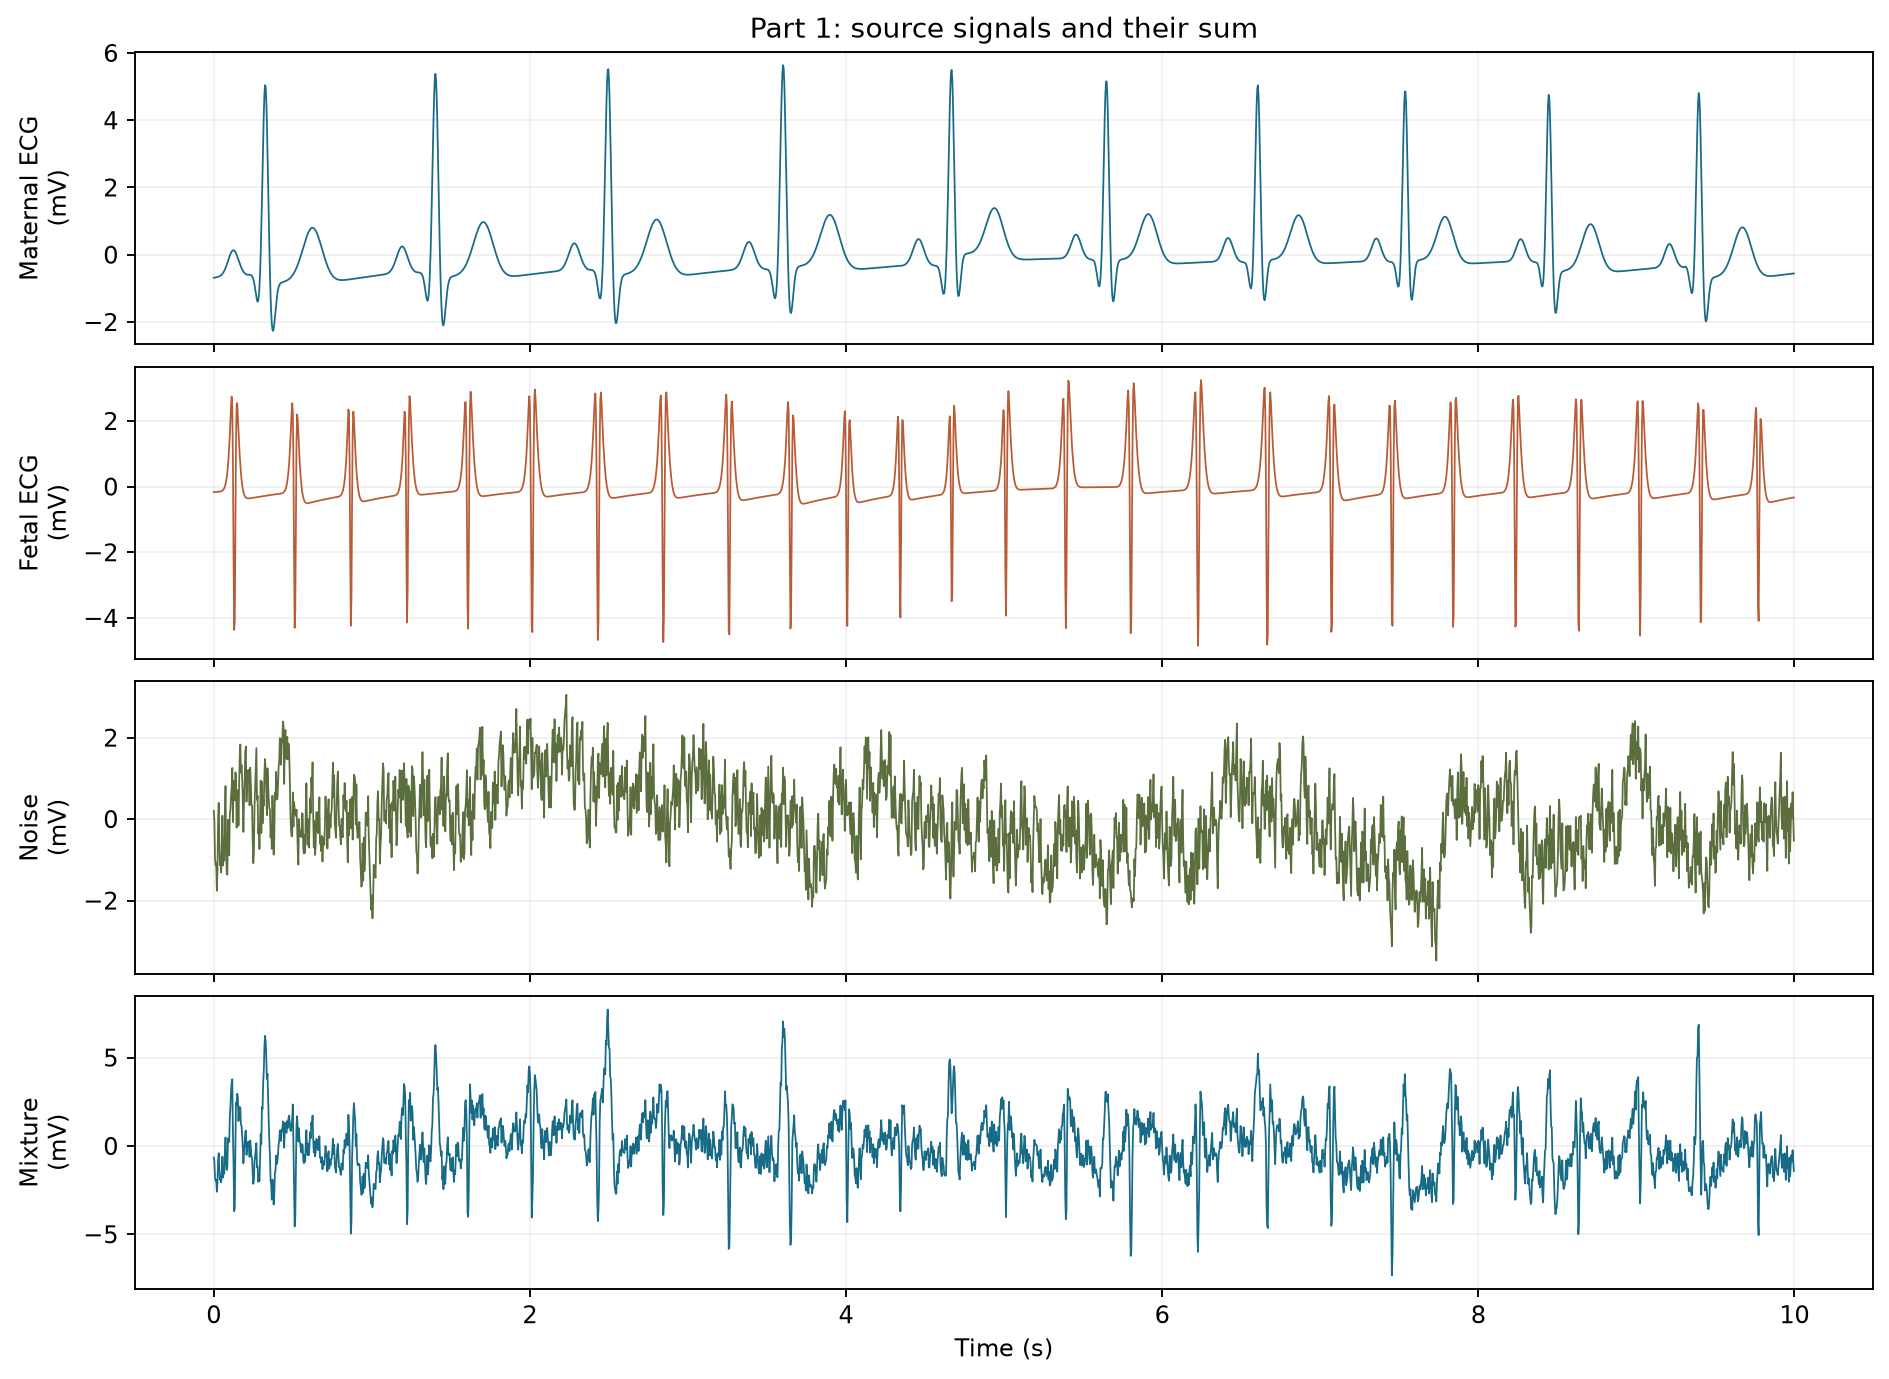
\includegraphics[width=0.95\textwidth]{fig15_full_sources_10s.png}
\caption{The full 10-second version of the sources and the mixture of Part~1; complements Question 1-1.}
\label{fig:fullsources}
\end{figure}

\begin{figure}[H]
\centering
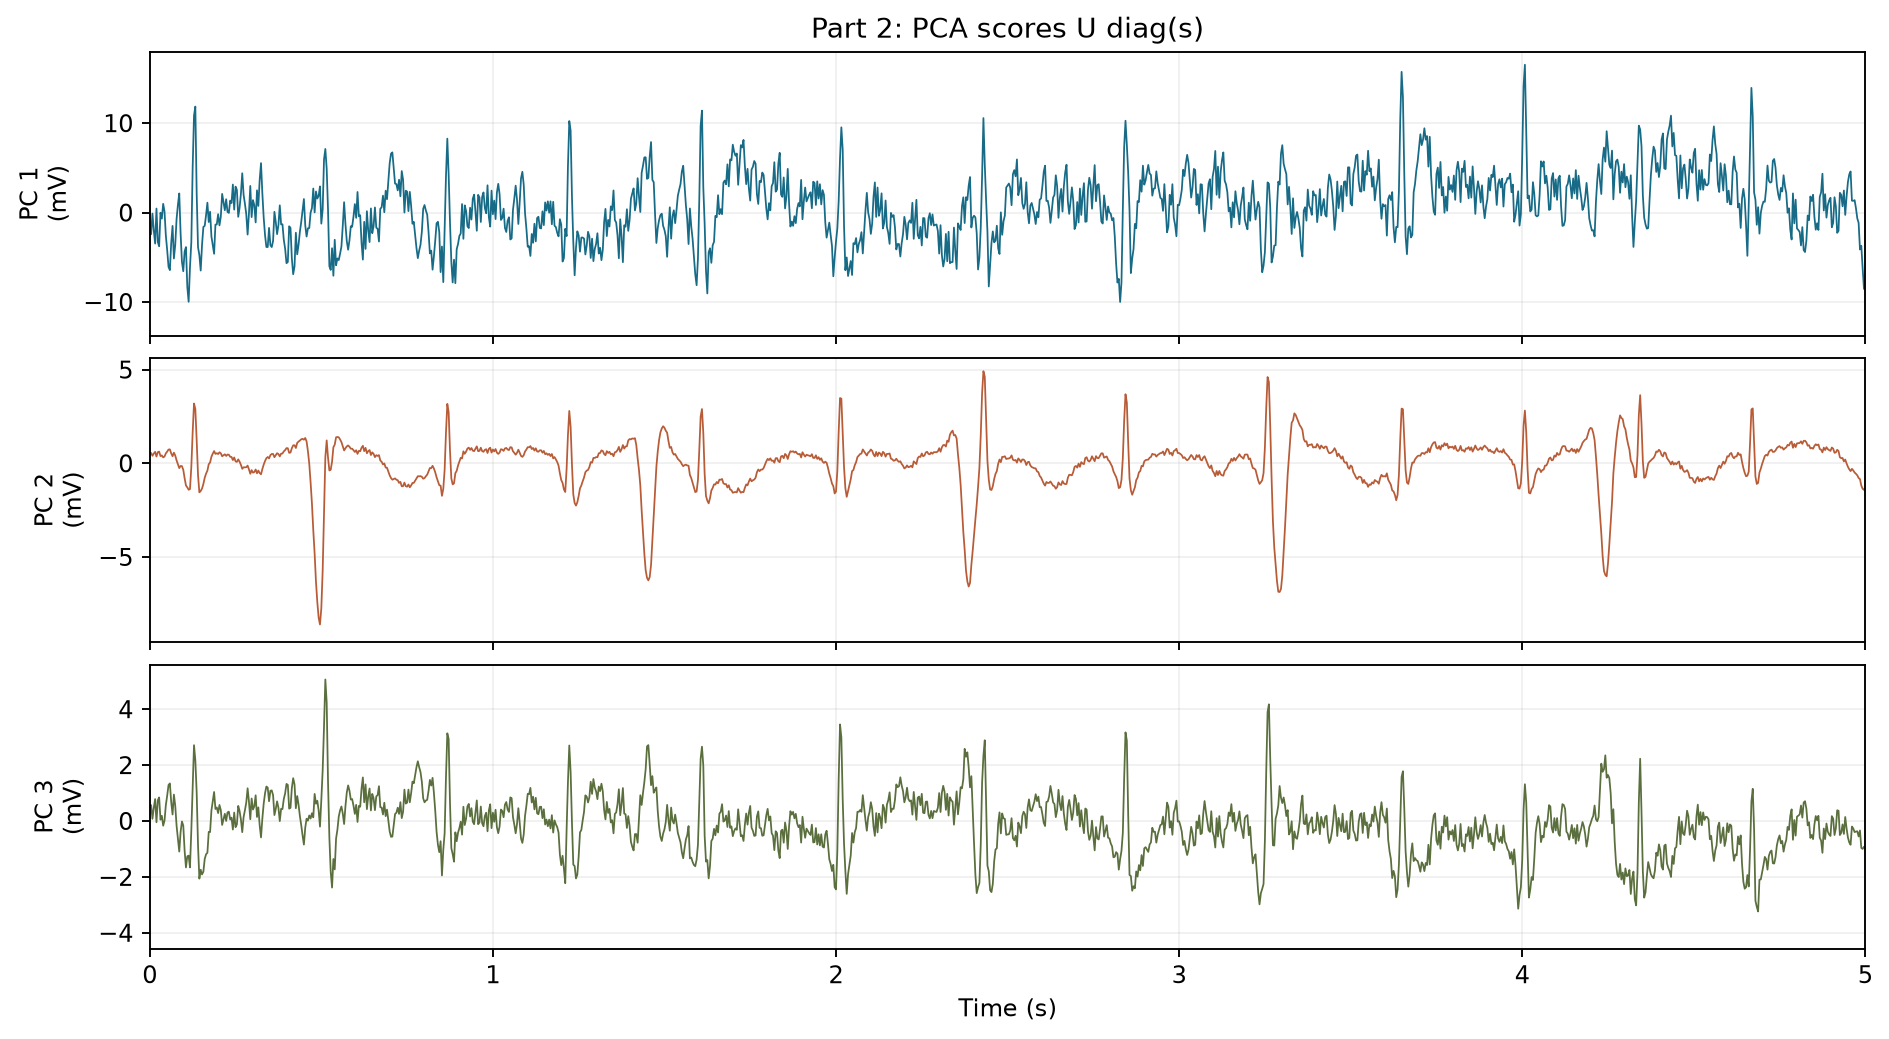
\includegraphics[width=0.95\textwidth]{fig16_pca_scores.png}
\caption{PCA scores, equal to $\mathbf{U}$ multiplied by the singular values; complements the normalized columns of $\mathbf{U}$ in Question 2-3.}
\label{fig:scores}
\end{figure}

\begin{figure}[H]
\centering
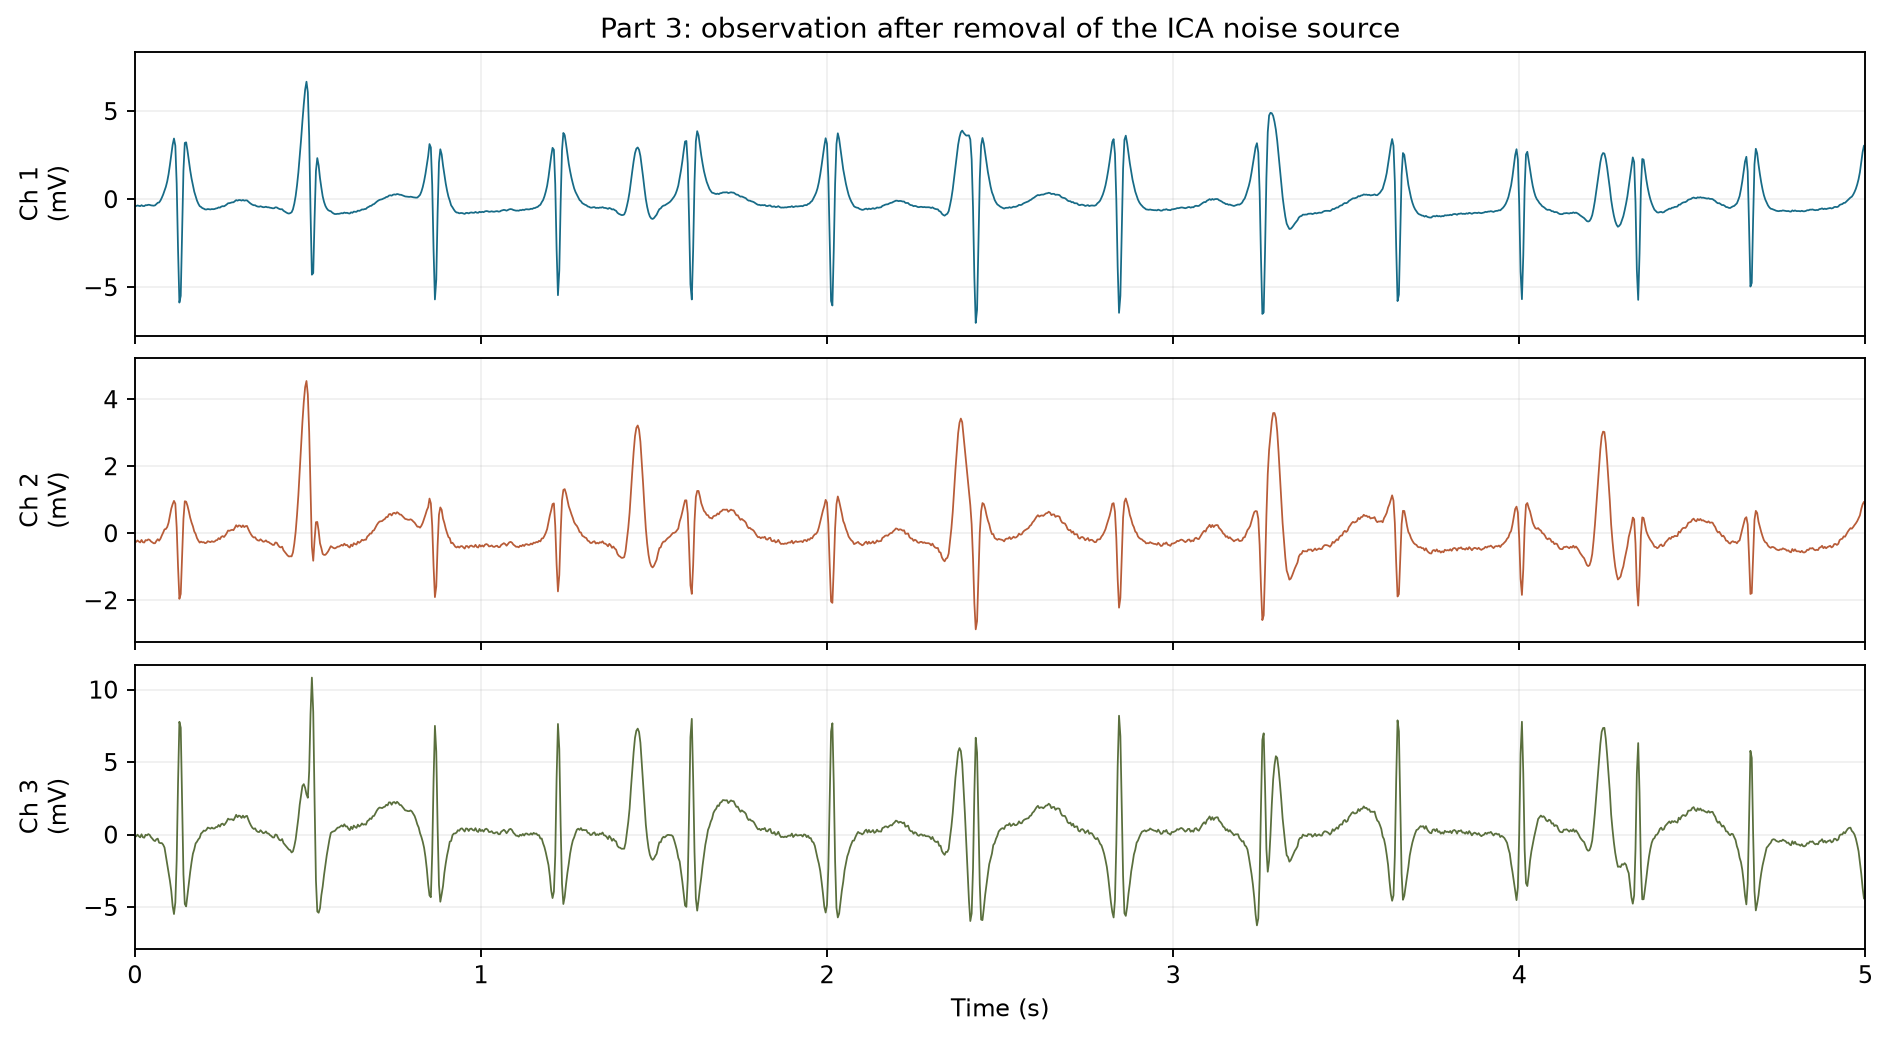
\includegraphics[width=0.95\textwidth]{fig17_ica_remove_noise_only.png}
\caption{Removal of only the contribution of the ICA noise component; the contributions of both the maternal and the fetal ECG remain.}
\label{fig:rmnoise}
\end{figure}

\begin{figure}[H]
\centering
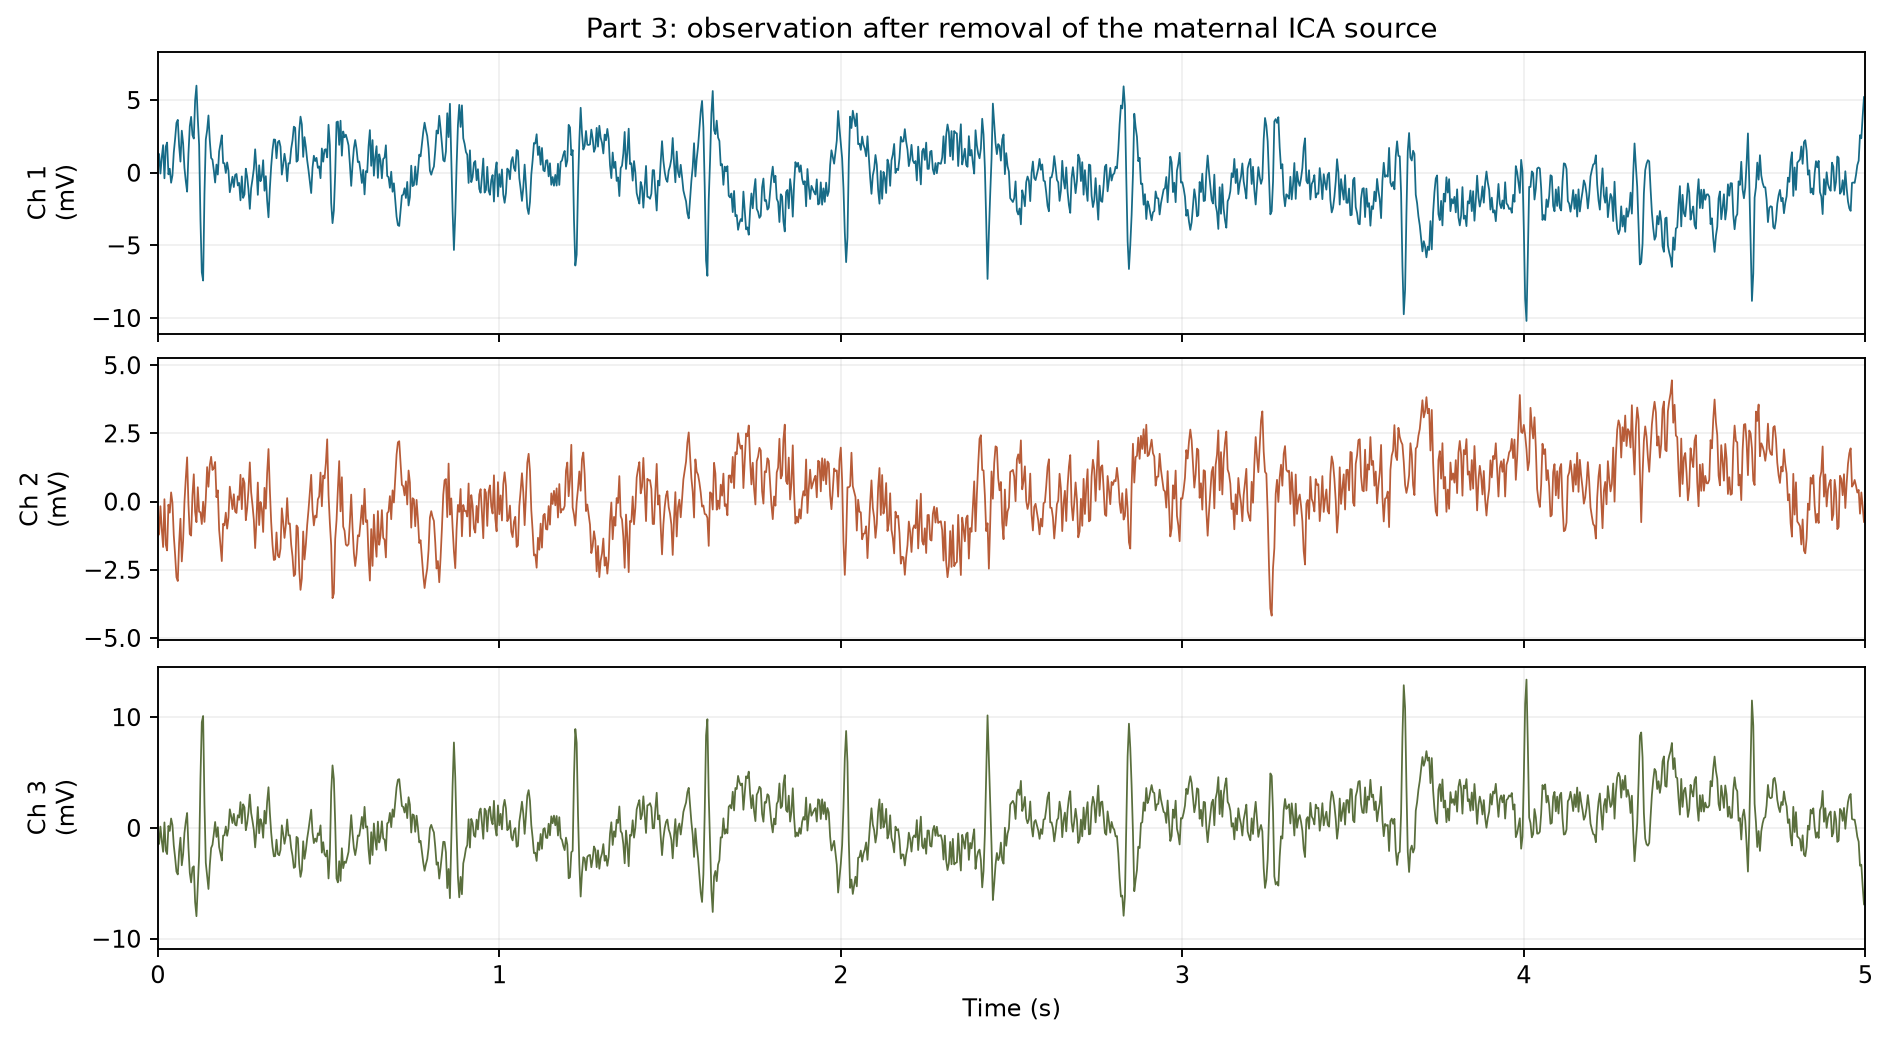
\includegraphics[width=0.95\textwidth]{fig18_ica_remove_maternal_only.png}
\caption{Removal of only the contribution of the ICA maternal component; the fetal ECG remains together with the noise.}
\label{fig:rmmat}
\end{figure}
